
\section{Online-PCA}

\mode<presentation>{
\begin{frame} 
    \begin{center} \huge
        \secname
    \end{center}
\end{frame}
}

\begin{frame}
W\notesonly{e have established that w}e can use Hebbian learning (Oja's rule to prevent divergence) 
to find the direction of the first \notesonly{principle component $\vec e_1$}\slidesonly{PC} in the data. \\

\pause

Note that with $\vec w = \vec e_1 \; \rightarrow \; y = \vec e_1^\top \vec x =: a_1$\\

\question{What else is there to do?}

\pause

- All other PCs

\end{frame}

\begin{frame}{Only}\frametitle{\secname}
\only<1-3>{
\svspace{-7mm}
\begin{center}
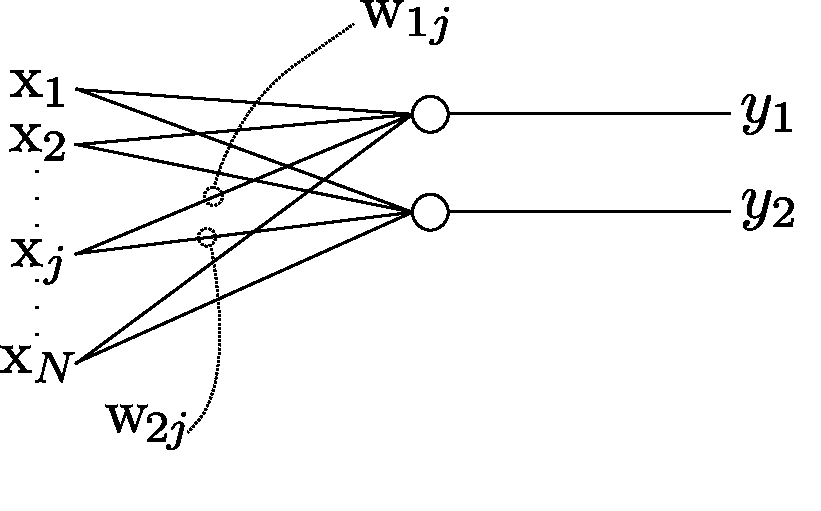
\includegraphics[width=4cm]{img/section2_fig5_b_2}
\svspace{-5mm}
\captionof{figure}{A neural network}
\end{center}
\svspace{-3mm}

We proceed to learning the next PC by doing the following:
}
\begin{enumerate}
\item<only@1-3> Denote the network's response with $y_1$ and its weight vector as $\vec w_1$, knowing that $\vec w_1 = \vec e_1$.
\item<only@1-3> Add a second neuron $y_2$ to our network. This neuron will come with its own randomly initialized weight vector $\vec w_2$.
\item<only@1-3,4> Resume feeding new data points into the network computing its response $y_1$ and $y_2$.
\item<only@4,5> We exploit the fact that the PCs form an \emph{orthonormal basis}, specifically, we obtain a projection of $\vec x$ 
into the subspace orthogonal to $\vec e_1$ that is the first PC:
\begin{align}
\hat x_j &= x_j - w_{1j} \, y_1 \\
         &= x_j - a_1 (\vec e_1)_j
\end{align}
where $w_{1j}$ is the weight of the connection between $\hat x_j$ and the neuron $y_1$,
\item<only@4-> Apply Oja's rule on $\vec w_2$.

For \emph{stationary data}: No need to apply updates to $\vec w_1$ anymore, since it has already converged to $\vec e_1$. Applying it to $\vec w_1$ will yields negligible change.
 
\item<only@4-> Continue feeding observations until $\vec w_2$ has converged.
\item<only@4-> On convergence, $\vec w_2 = \vec e_2$.
\end{enumerate}

\end{frame}

\begin{frame}

We get the remaining PCs by repeating the above except, that we project 
the data onto the subspace orthogonal to all previous PCs (cf. slides 1.2 \#12-\#14).

\end{frame}

\newpage

\section{Novelty filter}

Applying online PCA for detecting outliers - identifying observations with unusual features. 
Can also be done using ``standard``/batch PCA

\question{What are the PCs with smallest Eigenvalues useful for?}

\question{Can we modify online PCA by learning the PCs in reverse order (i.e. PCs with smallest eigenvalues first?}

\question{Is there an alternative way to learn a novelty filter? Under which assumptins does the alternative work?}

- (cf. slides 1.2 \#23-\#25.)

\section{PCA vs. online PCA}

\underline{Common properties:}

\begin{itemize}
\item assume the data is centered
\item sensitive to the scales of the individual variables
\item for stationary data, both converge to the same solution
\item limited to linear correlations between the variables (cf. Kernel PCA to account for non-linear correlations)
\end{itemize}

\question{PCA vs. online PCA. When do we use which?}

- staionarity of the data, can I fit all the data into memory?
